\hypertarget{blink}{%
\section{Blink}\label{blink}}

\hypertarget{overview}{%
\section{Overview}\label{overview}}

Blink is Loki's instant payment mechanism. It makes use of Loki's
service node layer and checkpointing mechanism to guarantee that a
transaction will eventually reach the blockchain without risk of various
adversarial attacks. This allows payments to be transferred almost
instantly from the point of view of a wallet while the loki nodes and
service nodes take care of the details of providing that guarantee.

This document discusses the design details of how Blink works.

\hypertarget{wallet-side}{%
\section{Wallet side}\label{wallet-side}}

From the user (wallet) side, initiating a Blink transfer is nearly
identical to initiating a normal transfer, but with an extra flag
(e.g.~GUI checkbox, RPC parameter, CLI option) to say ``Blink this
transaction!''.

The fees of the blink transaction are higher as it involves considerably
more work for the network: service nodes must validate the transaction,
and all nodes must perform extra validation steps and require some
temporary extra storage to store recent Blink transaction details.

For the user receiving a blink transaction, the wallet will see the
received amount virtually instantly (that is, as soon as it is received
by the lokid and the wallet refreshes with the daemon). Moreover these
funds will be instantly spendable: unlike a regular transaction there
will be no lock on the received funds before they can be spent again.
The wallet user can immediately re-Blink the funds to someone else, or
can send off a regular (non-Blink) transaction that spends the received
Blink outputs instantly without needing to wait for the Blink
transaction to be mined into a block.

\hypertarget{fees}{%
\section{Fees}\label{fees}}

The precise fee schedule is yet to be determined, but will be an
additional amount on top of the current transaction fee, most likely
calculated as a multiple of the transaction fee. Additionally, Blink
transactions will not have a choice in transaction priority: since they
are instantly spendable and guaranteed by the network, there would be
little point in a user ever choosing anything higher than the minimum.
Thus, for now, we mandate that Blink fees must always be submitted with
a ``normal'' priority transaction fee (but this is tentative and may be
adjust this before final Blink release).

The extra Blink fee doesn't go to anyone: rather it gets permanently
destroyed as part of the transaction. We considered two alternatives
here:

\begin{enumerate}
\def\labelenumi{\arabic{enumi}.}
\tightlist
\item
  Collecting fees and redistributing to SN over time. This is similar in
  notion to the current transaction fee paid to minersThis would involve
  temporarily burning Blink fees, but keeping track of how much had been
  burned and continually reemitting them over a period of time as an
  extra rewards to Service Nodes. (For example: in every block, reduce
  the current pool of burned fees by 0.1\% and reemit it to the service
  nodes that earn a reward in that block).
\item
  Just burning fees.
\end{enumerate}

Ultimately we decided on the second approach because:

\begin{itemize}
\tightlist
\item
  It is much simpler.
\item
  It is more predictable: SN rewards (for a stable number of service
  nodes) are known precisely.
\item
  In the end, the two approaches are effectively equivalent in terms of
  total emission.
\end{itemize}

By equivalent I am assuming that we have a specific net emission target.
For simplicity, I'll just talk about the long-term 28 LOKI/block
emissions, and, for the sake of example, assume that it is divided up so
that service nodes get 20 LOKI/block of that; the remaining 8 is
foundation and miner coinbase rewards. What I mean by net emission is
that if we have an average burning of 5 LOKI/block in Blink fees, then
the net emission is 23 LOKI/block. But let's suppose that 25 LOKI/block
is our actual desired emission target.

With method 1, we're emitting 28 LOKI/block: burned Blink fees are
reemitted over time and so, much like regular tx fees, there is no net
gain or loss. To hit the 25 LOKI/block target we'd have to adjust the
formula to reduce emissions to 25 LOKI/block.

With method 2, where we are burning 5 LOKI/block in fees, we are
generate net emissions of 23 LOKI/block; to hit the same 25 LOKI/block
target, then, we need to increase coinbase emissions by 2 LOKI/block.

Either way we arrive at the same place: net emissions of 25 LOKI/block
through adjustment of the emission schedule. And this was just an
example, of course; our actual target could be 20 or 28 or 12 or
whatever else. But with method 2, service nodes always know exactly what
they will earn, while with method 1 there is more variability: large,
sustained differences in the volume of Blink transactions will affect SN
profitability, while in method 2 such differences will affect the
overall coin emission but \emph{not} the amount earned by a service
node.

Thus, given the simpler approach and essential equivalence between the
two approaches, we decided to pursue method 2. (Of course, like anything
in Loki, we can always change the design later given compelling reasons
to do so!)

\hypertarget{transaction-overview}{%
\section{Transaction overview}\label{transaction-overview}}

In a nutshell (with most of the details covered later in this document):
The wallet builds a transaction and sends it to the lokid to be blinked.
The lokid then looks up the Blink quorum, connects to a few nodes in
this quorum, sending the transaction to them to be signed. The quorum
distributions the transaction within itself, and once enough approval
signatures are collected, broadcasts the transaction and signature data
to the service node's p2p peers to disseminate it across the network.
The lokid talking to the quorum then receives a confirmation message
(with signatures) to relay to the wallet.

These steps are depicted in the following diagram:

\begin{figure}
\centering
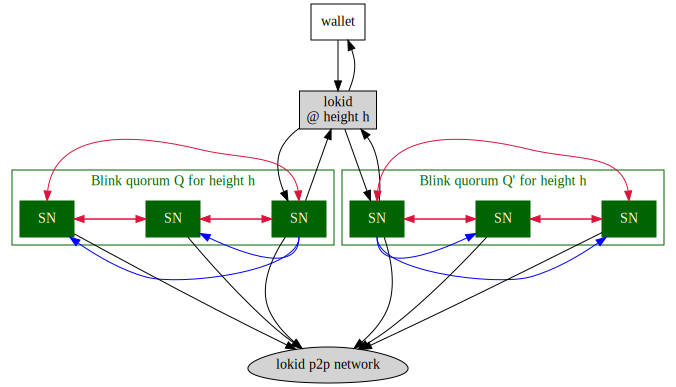
\includegraphics{blink.svg}
\caption{Blink tx flow}
\end{figure}

In more detail:

\begin{enumerate}
\def\labelenumi{\arabic{enumi}.}
\item
  The wallet constructs a transaction. This transaction is \emph{almost}
  like a regular transaction except that it leaves enough inputs unspent
  to cover both the required tx fee and the Blink fee. This transaction
  gets send to the wallet's lokid for handling.
\item
  lokid looks at the transaction, does some preliminary checks (as it
  would with any transaction) and an additional checks related to the
  Blink transaction (such as having the correct transaction priority and
  blink fee). These checks are not strictly required for network
  security---they will also be done by the service nodes---but can give
  an immediate failure response to the wallet if the node reasonably
  believes the transaction will fail. Assuming the preliminary checks
  pass, the node then uses the current blockchain height \emph{h} to
  build two quorums, \emph{Q₁} and \emph{Q₂} where \emph{Q₁} is the
  quorum for the current height and \emph{Q₂} for subsequent height
  blocks (more details on quorum construction below). lokid connects
  directly to 2 nodes selected randomly from each quorum and sends the
  transaction to be signed.
\item
  The receiving quorum nodes directly contacted by the initiating lokid
  forward the transaction to the other quorum nodes for verification.
\item
  Each service node in the two quorums performs much the same checks on
  the transaction as described above to determine whether the
  transaction is valid: i.e.~correct transaction structure, key images
  not already spent, and correctly specified miner and Blink fees. They
  also check whether the calling node's \emph{h} is approximately
  current (within 2 blocks of what the service node believes is the
  current height) and that the key images are not already locked out
  from a current Blink transaction in the mempool \emph{other} than the
  one in question. Assuming everything checks out, the service node
  records the transaction's key images locally (to lock them out from
  being used again within this quorum), signs the transaction hash with
  the service node private key, and sends the signature and public key
  to the other quorum members.
\item
  Once each of the quorum members has received a supermajority of valid
  signatures (i.e.~7 in total) from \emph{both} quorums it immediately
  sends out the transaction and signature details to its blockchain
  peers via its p2p network. If the quorum node in question is one of
  the nodes that was directly contacted by lokid, it communicates the
  success back to the caller.

  These signed mempool transactions, however, are much stronger than a
  regular mempool transaction in that they can trigger a reorg or lead
  to rejected blocks: more details on this are covered below.

  In the case of detectable failure (for example, from a detected
  double-spend confirmed by a sufficient number of service nodes), a
  failure message is returned to the caller. If a failure is caused by
  too many quorum nodes timing out the caller is expected to itself
  timeout after an appropriate amount of time waiting for a response.
\item
  The initiating lokid waits for success, failure, or timeout from the
  quorum nodes it contacted, and once received (or timed out), sends
  this information back to the wallet.
\end{enumerate}

\hypertarget{quorum-selection}{%
\section{Quorum selection}\label{quorum-selection}}

Quorum selection works by choosing two quorums, \emph{Q} and \emph{Q'},
for a height \emph{h} where each quorum is deterministic for a range of
5 blocks. So, for example, any 1000 ≤ \emph{h} ≤ 1004 will yield the
same \emph{Q} and \emph{Q'}. Moreover \emph{Q'} will be the quorum for
the immediately following set of 5 block heights. In other words,
\emph{Q'(height=1003)} and \emph{Q(height=1006)} are the \textbf{same
quorum}.

The quorum sample itself needs to be effectively immutable, and so we
propose a deterministic random sampling using a MT19937-64 random number
generator seeded with the block hash 35 blocks before the first valid
quorum height, \emph{h₀}. Thus quorum \emph{Q} for height 1002 is
determined by block 965 (35 blocks before the first height of the
quorum, \emph{h₀}=1000), and quorum \emph{Q'} is determined by block 970
(35 blocks before the first height of the second quorum,
\emph{h'₀}=1005). Moreover the sampling algorithm excludes any service
nodes that are scheduled to expire before block \emph{h₀}+10.

For validation of a Blink transaction we require a supermajority of
signatures from \emph{both} quorums. The point here is to prevent a
timing conflict where one Blink transaction is signed by quorum \emph{h}
and another, conflicting transaction is signed by quorum \emph{h+1}
\textbf{before} the \emph{h} transaction is broadcast to the network. By
using two overlapping quorums we end up with the key images in question
being locked from being spent in any other transaction for the next few
blocks: even if the next Blink transaction switches quorums, the overlap
ensures that it still must use a quorum that could have recent already
locked out some Blink key images.

All service nodes in \emph{Q} and \emph{Q'} refuse to sign a transaction
with a requested signing height more than 2 blocks behind or ahead of
the service node's current height: this is to allow some tolerance for
Blink transactions to succeed even if new blocks are propagating through
the network during the Blink transaction signing process. This ±2
tolerance is designed to make the user experience better: using a node
that is slightly out of sync\footnote{A node that is one minute behind
  the network will fall to more than 2 blocks away from the proper
  height 0.18\% of the time; with two minute lag the node will exceed 2
  blocks 1.89\% of the time; a thirty-second-slow node will be a problem
  0.013\% of the time. Since a node lagging by any of these values
  occurs only rarely (not consistently), the actual probability of users
  encountering such failures on a decently connected node should be much
  lower.} will still work fine rather than returning a Blink failure. It
also avoids potential Blink failures on the part of quorum nodes: if a
block happens to arrive during the actual signing process such that half
of the quorum see the new block and half see the old block the quorum
will still sign without issue.

\hypertarget{rationale}{%
\subsection{Rationale}\label{rationale}}

\hypertarget{overlapping-quorums}{%
\subsubsection{Overlapping quorums}\label{overlapping-quorums}}

There are three reasons for using these two overlapping quorums. First,
we want the quorum signature process to ``reach'' a few blocks into the
future (5--9 blocks ahead with 5-block quorums) to give enough time for
the quorum signatures to disseminate across the network. While 5 blocks
is more than would be typically required, there are some edge cases
discussed in detail below that can lower this future block interval to
just 2 blocks.

Second, Blink processing is expected to require a substantial number of
connections between service nodes; with 5-block quorums we can at least
reduce the frequency with which connections need to be established as
service nodes will keep their connections open for the duration of the
quorum.

Third, using two quorums offers considerable higher security than one
quorum of twice the size for two reasons. First, each quorum is
essentially a new random draw of service nodes; that means the more
quorums you have over a given period of time the more random draws you
do, and with more draws you get more ``chances'' to pick a compromised
sample. Second, two \emph{consecutive} supermajorities of quorums of
half the size is considerably more secure than one supermajority of a
quorum twice the size.

Some numbers can help demonstrate this: suppose the network has 1000
service nodes, and a single malicious actor is in control of 25\% of
those service nodes. Under alternative A, we require the majority of a
single quorum of 20 service nodes, and require a 70\% of the service
nodes' signatures. Under alternative B, we require two quorums of 10
service nodes each, again requiring 70\% signatures from each quorum.

Under scenario A in any given quorum the actor has a probability of
0.00000381 of having the required 70\% majority. Under scenario B, the
actor has a probability of 0.000000173: that is, under scenario A, the
actor is about 22 times more likely to obtain control of any random
quorum than any random quorum pair. Or to put it into context: in a one
year span, there's about an 18\% chance that this bad actor would gain
quorum control for at least a single quorum under scenario A, and about
a 0.9\% chance that he would under scenario B. As for quorum length, if
quorums lasted for one block instead of five there would be a 4.4\%
chance of this 25\% operator having a quorum supermajority at least once
under the overlapping quorum design, and a 63\% chance under the single
quorum design.

If this adversary actually controlled an incredible 50\% of the service
node network it would be quite difficult to avoid a compromise: he would
have quorum supermajority votes about 2\% of the time under the single
quorum approach, and 0.3\% of the time under the overlapping quorum
approach. Such an adversary would have a 95\% chance of quorum ownership
at least once \emph{per day} with a quorum of 20, and a 35\% chance per
day with overlapping quorums. On the other hand, the economic design of
Loki makes this case less worrying: even if such adversaries existed,
they would have a strong financial incentive to ensure that the network
is not compromised.

There is, of course, some desirable statistical properties of making a
quorum \emph{longer}: if quorums changed on a 10 block cycle you'd cut
the probability of compromise by nearly half (to 0.45\% in the
overlapping case). This gain isn't huge, though; moreover the longer the
quorum becomes the more complications can arise from service node
deregistrations, and the more time you allow for coordination between
service node operators looking to cheat the system.

Instead, if we wanted to further increase the security of Blink
transactions, a preferable approach would be to use a triple quorum. It
could also be possible to enable an opt-in triple quorum, at a higher
fee, to allow users to send with a paranoid level of assurance. (This is
now, however, part of the current Blink plan.)

\hypertarget{quorum-selection-block-and-checkpointing}{%
\subsubsection{Quorum selection block and
checkpointing}\label{quorum-selection-block-and-checkpointing}}

Using a lag of 30 blocks for quorum determination was chosen to interact
with Loki checkpointing. Unlike checkpointing and deregistration
quorums, a change in Blink quorums would be highly undesirable as the
validity of the Blink signature would no longer hold. Thus we want to
use a height from the blockchain that is sufficiently far back as to be
highly likely to be made immutable via checkpointing. By basing the
quorum on \emph{h₀}-30 we give ample time for checkpointing even if 2-3
checkpoints have been missed.

For example, if blinking at height 1000 then \emph{Q'} begins at 1005,
which means the relevant block for determination of \emph{Q'} is 975.
Checkpointing normally occurs every 4 blocks with immutability occurring
after 3 checkpoints. Thus in typical times it can be up to 4 blocks
since the last checkpoint quorum, which itself establishes a checkpoint
on a block 4 blocks earlier. Allowing up to 2 blocks for the quorum to
vote and disseminate the checkpoint to the network this means the first
checkpoint is usually between 4 and 10 blocks ago, the second is 8-14
blocks ago, and the third, immutable checkpoint is 12-18 blocks ago. If
one of these checkpoints were missed (for example because of a quorum
failure) then the immutable checkpoint could be 16-22 blocks ago; and if
three were missed, up to 30 blocks ago. Thus the \emph{h₀}-35 rule
establishes that both quorum selections are established by a block at
least 30 blocks in the past, which allows Blink to tolerate up to 3
missing checkpoints.

To further secure Blink transactions we further require that the quorum
seed heights are checkpoint-immutable: both the initiating lokid and the
quorum service nodes will verify that the quorum seed height is in fact
checkpointed, refusing to sign (and thus failing the Blink if enough
fail to see the required checkpoints) if it is not. This ensures that
Blink transactions are secure by preferring to fail a Blink signature
rather than include one that has any chance of being invalidated by a
block reorganization.

\hypertarget{quorum-validation}{%
\section{Quorum validation}\label{quorum-validation}}

Some potential cases are depicted below:

\begin{figure}
\centering
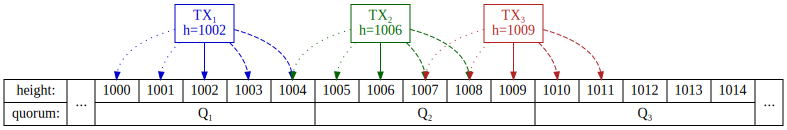
\includegraphics{quorums.svg}
\caption{Transactions and quorums}
\end{figure}

\hypertarget{tx-example-one}{%
\subsection{TX example one}\label{tx-example-one}}

\emph{TX₁} is depicting a transaction submitted to a daemon which sees
the current height of the network at 1002. We can think about a few
different cases:

\begin{itemize}
\item
  Submitting the blink transaction normally at the known height (1002).
  Thus we get \emph{Q = Q₁} and \emph{Q' = Q₂} for the two quorums. The
  initiating lokid contacts a random service node \emph{q} from
  \emph{Q₁}, passes along the transaction, and waits for a reply from
  \emph{q}. \emph{q} in turn communicates with its quorum peers and the
  subsequent quorum (\emph{Q₂}) to build the required set of signatures.
  Once the required signatures are accumulated the transaction is
  released by the quorum service nodes to their peers.

  The Blink TX is broadcast to the network. Because a majority of
  \emph{Q₂} service nodes signed it and will not resign the same key
  images, the earliest possible Blink height to spend the same key
  images is 1010, which can be used by a cheating lokid at network block
  1008 at the earliest.
\item
  Submitting slightly behind the network (1000 or 1001). This could
  happen, for instance, because there have been two recent blocks that
  the local lokid has not synchronized yet. Generally everything here
  works as above: the service nodes at height 1002 will still sign the
  block (assuming the transaction itself is valid) because the requested
  signature height is within 2 of their current height.
\item
  Submitting slightly ahead of the network (1003 or 1004). This could
  happen, for instance, if the local node is close to a very lucky pool
  that has just discovered a couple blocks that haven't disseminated
  across the network yet. Again, this is handled just like the above:
  even though the service nodes haven't yet seen a block newer than 1002
  it still satisfies the within-2 rule and so they will still sign
  (assuming the transaction is valid).
\item
  Submitting well behind or well ahead of the network (999 or lower, or
  1005 or higher). In this case the quorum will not accumulate enough
  signatures because the within-2 requirement is violated. In this case
  a failure gets returned to the initiating lokid.\footnote{It is
    possible for the quorum to return an error status indicating that
    the lokid should retry at a new height; it is up to the lokid
    whether it wants to do this or return an error to the client.}
\end{itemize}

The first three (accepted) cases above all result in the earliest block
a cheater could submit to being 1008 (i.e.~abusing the within-2 rule to
submit a h=1010 block), giving a worst case of at least 4 blocks needing
to be transmitted to the network before a duplicate Blink could be
submitted; since Blink dissemination is high-priority this should result
in a high level of assuredness that a Blink double-spend cannot be
performed in this scenario.

\hypertarget{tx-example-two}{%
\subsection{TX example two}\label{tx-example-two}}

\emph{TX₂} shows a transaction that is sent via a lokid that sees the
current \emph{h=1006}, i.e.~in the second block of quorum \emph{Q₂}.
I'll just ignore the \emph{h\textgreater{}1008} and
\emph{h\textless{}1004} cases (see above for why they are dead ends).

\begin{itemize}
\item
  Case 1: Submitting \emph{h}=1005, 1006, 1007, 1008. This case is
  largely the same as \emph{TX₁}, but now the two quorums are \emph{Q₂}
  and \emph{Q₃}. The earlier a theoretical double-spending Blink could
  be submitted is with \emph{h}=1015 at actual height 1013: that is, a
  minimum of 5 network blocks away.
\item
  Case 2: Submitting \emph{h}=1004 (either due to a lagging node, or a
  malicious actor). This ends up using the same quorums as \emph{TX₁}
  (that is, \emph{Q₁} and \emph{Q₂}). As in \emph{TX₁}, the earliest
  possible double spend could be submitted at 1008.
\end{itemize}

Case 2 here represents the worst possible scenario: there are just two
network blocks between the current height (1006) and the height at which
a blink transaction could be submitted to a completely independent
quorum pair. There is a potential issue here from an attacker, discussed
in further detail below.

\hypertarget{tx-example-three}{%
\subsection{TX example three}\label{tx-example-three}}

\emph{TX₃} is included for completeness to show that cheating
\emph{ahead} by a quorum has no advantage for a potential attacker. This
depicts the sending transaction at \emph{h}=1009. The attack essentially
has two relevant choices: \emph{h}=1007--1009, or \emph{h}=1010,1011. In
the first case, he gets quorums \emph{Q₂} and \emph{Q₃}, making his
earlier possible Blink double-spend at \emph{h}=1015 (submitted at
\emph{h}=1013), which is

Stats geek note: the probability of being 3+ blocks behind the network
with lag \emph{L} seconds is the CDF value of a Poisson distribution
with λ=\emph{L}/120 at \emph{k}=3.

\hypertarget{signature-failure-key-images-may-stay-unblinkable-for-up-to-10-blocks.}{%
\section{Signature failure: key images may stay unblinkable (for up to
10
blocks).}\label{signature-failure-key-images-may-stay-unblinkable-for-up-to-10-blocks.}}

When a service node signs a transaction as part of a given quorum it
will never sign a different transaction containing any of the same key
images again as part of that quorum. Since failures are possible for
multiple reasons, however, it does not block the key images of a
transaction that it refused to sign.

It is possible, however, for a transaction to fail to be signed by a
supermajority while still being signed by a superminority (that is, by
enough other nodes to prevent a supermajority). This case is expected to
be rare: the criteria for service node disagreement is small:
effectively you would need (roughly) half of the service nodes to see
something wrong with the transaction. It is not impossible, however: if
a regular transaction spending the same key images is mined and the
block transmitted in the middle of signing the blink could fail.

The user-facing problem that could arise here is that the transaction
that gets signed includes multiple key images, only some of which are
ineligible. The service nodes that signed the transaction, however, end
up locking \emph{all} of the key images for the duration of the quorum (
i.e.~the next 4--9 blocks), so even once the user wallet sees the
updated chain a new transaction \emph{might} end up trying to blink
using an input that is temporarily non-blinkable (note that it
\emph{will} still be regularly minable since the Blink was not
transmitted due to the quorum failure).

This case seems rare: it would require a legitimate user spending
regular transactions and blinking at the same time from different
wallets. It's possible, of course, but given the rarity and the
relatively minor consequence (not being able to Blink those outputs for
10--20 minutes) for now we will simple leave this as a known limitation.

\hypertarget{blinked-transactions-in-the-mempool}{%
\section{Blinked transactions in the
mempool}\label{blinked-transactions-in-the-mempool}}

Blink transactions themselves are perfectly ordinary transactions on the
blockchain: the signatures applied by service nodes do \emph{not} end up
as part of the transaction that gets mined into the chain. Instead this
metadata is shared and synchronized between nodes from the time when a
Blink transaction enters the mempool until the transaction is mined
\emph{and} secured behind an immutable Loki checkpoint boundary.

An incoming Blink transaction in the mempool will also be transmitted
with the Blink height and the verifiable Blink signatures at which the
transaction was signed. Based on this, a loki node receiving a blink
transaction will perform multiple actions:

\begin{itemize}
\tightlist
\item
  verify that the Blink signatures are the correct signers for the given
  height, and that the signatures are valid (and if not reject the Blink
  transaction).
\item
  check to see if any of the key images were spent in or before the last
  irreversible checkpoint block: if so, reject the Blink transaction.
\item
  check to see if the mempool already contains any Blink transactions
  that have a higher priority (i.e.~lower height) than the incoming
  transactions, and if so, refuse the incoming transactions. (This
  shouldn't be possible, but is included as a safeguard to maintain
  consensus).
\item
  check the current chain back to the last irreversible checkpoint: if
  any blocks contain any transactions that spend any of the key images
  in the new Blink transaction then roll back the chain as much as
  needed to remove those transactions from the blockchain, re-adding any
  rolled back transactions into the mempool (as occurs already with any
  reorg).
\item
  reject any non-Blink transaction from the mempool that spend the same
  key images as the new Blink transaction (if we just rolled back then
  this means immediately rejecting the conflicting transactions).
\item
  reject any \emph{Blink} transactions from the mempool that spend the
  same key images but have a lower priority (i.e.~higher height) than
  the new Blink transaction. This should not be possible in general, but
  needs to be specified anyway to avoid a consensus failure (as with the
  mirrored check above). Note that this actual removal could cascade if
  there are other transactions referencing the removed Blink
  transaction.
\end{itemize}

Another difference with Blink transactions is that they should not be
subject to the existing 2-week mempool transaction timeout. We don't
want someone to be able to submit a low-priority Blink transaction while
the network is flooded with higher priority transactions and be able to
wait out the transaction until timeout. As long as Blink transactions
stay in the mempool until mined all an attacker can do is delay the
transaction from being mined, but cannot cause it to be dropped no
matter how long he prevents mining. In the unlikely event of a bug that
makes a Blink transaction inadmissible to the blockchain for some
unforeseen reason, this approach will keep the transaction alive
indefinitely until the bug can be addressed.\footnote{This is actually a
  bit more complicated because new transactions can be submitted that
  spend the Blink transaction outputs or that include the Blink
  transaction outputs as a decoy. That means those transactions
  themselves will depend on the Blink transaction, adding further
  chaining.}

Second, Blink transactions need to be more actively propagated across
the network than current transactions. Currently the mempool is not
actively synchronized across nodes; instead new transactions are simply
broadcast to all connected peers when received. A new node, a node that
was temporarily down when the transaction propagated across the network,
or a node that has had its mempool manually flushed does not receive
existing mempool transactions from peers if it misses it the first time.
This needs to change for Blink transactions: when a p2p connection is
established we need each peer to send the other a list of any pending
Blink transaction details it doesn't already have. Effectively we need
Blink transactions in the mempool to become first-class synchronization
objects, just like blocks.

\hypertarget{blinked-transactions-into-the-blockchain}{%
\section{Blinked transactions into the
blockchain}\label{blinked-transactions-into-the-blockchain}}

A transaction entering the blockchain from the mempool requires two
changes: first, the Blink transaction's unspent amount now includes both
the tx fee, as before, but now \emph{also} the Blink fee. Second,
because transactions can reference other Blink transactions currently in
the mempool this puts an ordering on transactions: if A includes B in
its ring signatures (whether as the actual key image or a decoy) then
there is an implied ordering for mined block selection: A cannot be
included in a block before the block in which B is included. This
requires, of course, changes to the transaction selection algorithm used
to construct block templates for miners.

\hypertarget{re-blinking}{%
\section{Re-blinking}\label{re-blinking}}

Blink needs the ability to ``re-Blink'' for an effective user
experience. That is, we want a Blink transaction to be instantly
available to the recipient indistiguishable from a (confirmed) non-Blink
transaction. For example, when Ava blinks 10 LOKI to Betty then that
transaction is initially still in the mempool, but we don't want Betty
to have to worry about this technical detail.

That means, however, that Betty should be able to spend those received
funds immediately, whether in a new non-Blink transaction or in a new
Blink transaction. In either case this means the new transaction will
spend outputs that aren't yet on the chain, but are still in the
mempool. We need to update lokid and the wallet allow this.

This does, however, raise another issue, addressed in the next section.

\hypertarget{ring-signature-implications}{%
\section{Ring signature
implications}\label{ring-signature-implications}}

The anonymity in Loki depends on the actual and decoy outputs being
included in the transaction ring signature being indistinguishable.
Quick turn-around \protect\hyperlink{re-blinking}{re-blinking} breaks
that with the current ring signature selection in two ways:

First, a Blink transaction that enters the mempool that includes a
mempool Blink transaction in its ring signature provides a perfect link
between the transactions because currently only blockchain transactions
but not mempool transactions are ever included in a ring signature.

Even if you don't have the mempool history you can still infer likely
links between Blink transactions that are very close together
(i.e.~within a small number of blocks). As outputs in the same block (or
within a couple blocks) are highly unlikely to occur naturally, seeing
such transactions in the mempool give a high probability that the
transactions are linked.\footnote{Effectively the only way to get a tx
  in block \emph{h} that refers to a tx in block \emph{h} or \emph{h-1}
  is if a blockchain reorganization that dumps transactions back into
  the mempool happens; this typically only occurs in a 51\% attack so
  can be considered rare enough to provide a high assurance of the link
  between transactions.}

To get around this problem, we will need to update the ring signature
construction to be able to select from both existing blockchain
transactions \emph{and} Blink transactions in the mempool for both Blink
transactions \emph{and regular transactions}. (This of course imposes
additional mempool ordering constraints to those discussed in the
{[}blockchain{]}{[}\#blinking-at-the-blockchain{]} section as ordering
also applies to non-Blink transactions using mempool decoys.) Further
investigation will be needed to determine a good selection probability
(and will likely need tweaking in future releases), but we will aim to
be on the side of having too high a probability: using too \emph{low} a
probability is much worse as it would make Blink transactions still
stand out (albeit imperfectly).

Potentially including mempool Blink transactions in normal transaction
ring signatures is important as well: because a Blink transaction is
instantly spendable, a non-Blink transaction including a recent Blink
transaction would similarly link the outputs together. Thus we
potentially include Blink dummy transactions in \emph{all} transactions
(which has the separate advantage of simplifying the code: building a
Blink transaction and building a regular transaction will be identical).

\hypertarget{blink-and-checkpoints}{%
\section{Blink and checkpoints}\label{blink-and-checkpoints}}

Blink transaction metadata (i.e.~quorum signatures, signing height) is
meant to be temporary data that only needs to be kept until the
transaction is unequivocally committed to the blockchain. Thus Blink is
designed to work with Loki's checkpointing feature: once the transaction
has passed the point where it is not reversible---that is, once it has
been signed by three checkpoint quorums---service nodes can discard the
metadata.

\hypertarget{quorum-communication}{%
\section{Quorum communication}\label{quorum-communication}}

Current quorum communication (e.g.~for deregistration voting or for the
upcoming checkpointing support) relies on a gossip protocol to carry
messages over the loki p2p layer. While this is manageable for those
applications it is not going to be sufficiently scalable for Blink
quorum voting.

Instead part of the Blink development will be to build a direct
communication layer where service nodes connect directly to one another
for quorum purposes. The initial plan is for quorum SNs to communicate
directly with each (using the SN public IP being added in
\href{https://github.com/loki-project/loki/pull/622}{\#622}). This
communication layer will also be designed to handle quorum traffic for
service node deregistration and allow faster and more efficient
communication in those scenarios as well.

The specific implementation details will be developed further during the
Blink implementation; the current plan is to create a relatively simple
SN-to-SN protocol using ZMQ (which is already a loki core dependency)
over which quorum members communicate, and over which the initiating
lokid contacts quorum service nodes to begin the Blink signing process.
The initial approach here is to use a fully-connected quorum: 9 open
connections, roughly half inbound and half outbound, for each SN, held
open (and reestablished upon disconnection) for the duration of the
Blink quorum validity.

As a simple fully connected approach, the following table shows
node-to-node connections within a quorum:

\begin{figure}
\centering
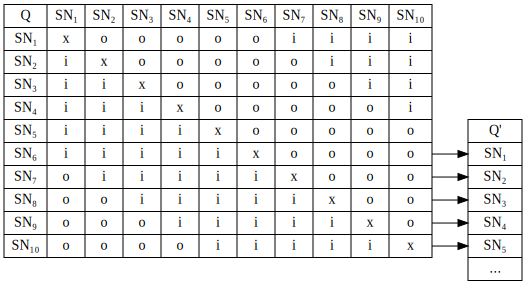
\includegraphics{blink-quorum-conns.svg}
\caption{Node-to-node quorum connections}
\end{figure}

where ``o'' indicates that the row node establishes an outgoing
connection to the column node and ``i'' indicates that the row node
receives an incoming connection from the column node. Additionally once
the depicted quorum Q becomes the first quorum, nodes 6--10 establish
outgoing connections to nodes 1--5 of following quorum, Q'. (Similarly,
but not depicted, when Q is the second quorum there will be inbound
connections to SN₁ through SN₅ from the previous quorum's last 5 nodes):
first node in the quorum will open connections to nodes 2--6, the second
node will open to nodes 3--7, and so on. The sixth node will open
connections to nodes 7--10, the seventh node to 8--10 and 1, and so on.
Additionally, once a quorum becomes the first quorum, nodes 6--10 each
establish a connection to nodes 1--5 in the second quorum.

Additionally, each quorum would have some nodes that establish a
connection to some of the nodes in the following quorum over which
messages will be passed when a quorum has acquired the required
supermajority of signatures.

\hypertarget{potential-attacks}{%
\section{Potential attacks}\label{potential-attacks}}

While the basics of the above in normal operation are fine, there are
several edge cases that need to be addressed specifically to prevent
accidental conflict or deliberate attacks.

\hypertarget{double-spending-blink-tx-non-blink-tx}{%
\subsection{Double-spending Blink tx + non-Blink
tx}\label{double-spending-blink-tx-non-blink-tx}}

This attack would work by privately mining a block where the inputs used
in a Blink transaction are spent, conducting a Blink transaction, then
releasing the private block to the network after the Blink transaction
has been approved. This would be a classic double spend, but because
Blink transactions are 0-confirmation transactions, you don't need a
51\% attack; you would just need a single block and a bit of luck.

The solution to this is that Blink transactions \emph{in the mempool}
are stronger for consensus purposes than non-Blink transactions \emph{on
the chain}. That is, if a Blink-signed transaction arrives in the
mempool that conflicts with (i.e.~spends the same inputs as) a
transaction already mined on the chain then the block containing the
conflicting non-Blink transaction is \textbf{no longer} a valid
blockchain block and must be rolled back.

There is a limitation to this, however: if the conflicting block has
passed an irreversible checkpoint boundary then it is instead the Blink
transaction that is invalid.\footnote{This case is virtually impossible
  in normal operations, but it must still be specified and handled for
  completeness of consensus rules.}

\hypertarget{double-spending-blink-blink}{%
\subsection{Double-spending Blink +
Blink}\label{double-spending-blink-blink}}

Sending two parallel Blink transactions that spend some of the same
inputs at the same signing height \emph{h} isn't possible: the approving
service nodes by design will not sign twice for the same outputs, and to
actually be accepted a Blink transaction must be signed by a
supermajority of the service nodes in the (unique) signing quorum.

Sending two Blink transactions at different heights, however, can be a
potential issue if exploited by something I will call ``quorum hopping''
and address in the next section.

\hypertarget{quorum-hopping}{%
\subsection{Quorum hopping}\label{quorum-hopping}}

In order to double-spend Blink transactions it is necessary to ``quorum
hop'' -- that is, to have your transaction signed by two independent
sets of quorums. Practically speaking, that means that that you need one
Blink transaction signed by \emph{Q₁} and \emph{Q₂}, and another
spending the same outputs signed by \emph{Q₃} and \emph{Q₄}.\footnote{You
  could hop further, of course, to \emph{Q₄} and \emph{Q₅}, but the
  attack is the same: it is just more costly to pull off.}

For the purposes of illustration, I'll continue with
\protect\hyperlink{tx-example-two}{TX example two}, and I'll assume the
attacker has an arbitrary amount of hash power available. In order to
quorum hop, the attacker needs to get signatures from \emph{Q₁} and
\emph{Q₂} \textbf{and} signatures for another transaction spending the
same outputs from \emph{Q₃} and \emph{Q₄}. The basic assurance is that
while the current network is at height 1006, \emph{Q₄} won't sign a
transaction. However, 1006 is close enough to the quorum endpoint that
the attacker does get a choice between the \emph{Q₁/Q₂} pair and the
\emph{Q₂/Q₃} pair: though \emph{Q₂/Q₃} is the proper quorum pair for a
truthful \emph{h}=1006 request, we allow him to claim \emph{h}=1004 (to
allow for network latency).

To get a successful signing from the \emph{Q₃/Q₄} quorum pair, however,
the second Blink transaction must request a signing height of at least
\emph{h}=1010, and the quorum won't accept such a height unless it
locally sees at least \emph{h}=1008. This means the attacker needs to
get two need blocks on the network quickly but not too quickly: if too
fast, the transaction may reach too many of the \emph{Q₁/Q₂} quorum
members that the first tx signature fails. If too slow, the signed
transaction broadcast from \emph{Q₁/Q₂} service nodes may reach enough
\emph{Q₃/Q₄} service nodes that signing of the second transaction fails.
Thus we'll assume that there is some small window for ``goldilocks''
timing: timing that is not too fast to reach \emph{Q₁/Q₂} and not too
slow to reach \emph{Q₃/Q₄} after the first transaction.

The timing of the attack would go like this:

\begin{enumerate}
\def\labelenumi{\arabic{enumi}.}
\tightlist
\item
  Privately mine and withhold 2 blocks (heights 1007 and 1008).
\item
  Initiate a Blink signing at \emph{h}=1004 (thus using the \emph{Q₁/Q₂}
  quorum pair).
\item
  Release the withheld blocks; ideally send them directly to
  \emph{Q₃/Q₄} quorum members.
\item
  Initiate the conflicting transaction Blink signing at \emph{h}=1008
  (thus using \emph{Q₃/Q₄}).
\end{enumerate}

If successful, nodes on the network will end up receiving two conflict
Blink transactions with valid signatures. First, for a unique consensus
rule, we need to pick a consensus winner, which is easy enough: we
simple prefer the Blink transaction with an earlier signing height and
reject the later one.\footnote{In theory there could be transactions
  that reference the second transaction's outputs that would also need
  to be ejected from the mempool. Given that the window of opportunity
  here is extremely small, this seems a negligible concern.}

Second, and more important, we want to make the attack to be
``impossible''\footnote{In a practical sense, of course. More
  technically, we want the attack to be extremely difficult to carry
  out.}. This is done by effectively adding a delay to Blink signing in
potentially problematic case, effectively shortening the ``goldilocks''
window to nothing. Specifically the proposed delay is as follows: when a
quorum service node is asked to sign a transaction at height \emph{h},
it checks the time when it received the critical block that allowed the
given quorum pair associated with height \emph{h}. If this critical
block was received less than 5 seconds ago, it delays the Blink checks
and signing until at least 5 seconds have elapsed since that critical
block was was received by the given service node.

For example, the critical block for a signing height of 1007 would be
1003; for 1010 it would be 1008:

\begin{figure}
\centering
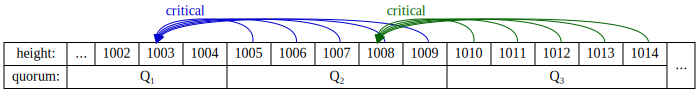
\includegraphics{quorum-critical.svg}
\caption{Quorum critical blocks}
\end{figure}

The whole idea here is to add enough of a delay that the Blink
transaction being signed by \emph{Q₁/Q₂} has time to propagate to enough
\emph{Q₃/Q₄} service nodes that they will see the double-spending
attempt and thus fail to build enough signatures to Blink the
transaction. 5 seconds should generally be much more than enough for
reach all the quorum members, but we don't actually need it to reach
all: rather it is enough to reach just a supermajority-busting minority
or \emph{either} \emph{Q₃} or \emph{Q₄} service nodes.

A delay of up to 5-seconds is highly undesirable for a Blink
transaction, of course, so it is worth considering how unlikely this
delay would be under typical blockchain activity when an honest user is
sending a Blink transaction.

Let's suppose the user submits a transaction to sign at height
\emph{h=1010}, and so quorum service nodes check when they received
block \emph{h=1008} to figure out whether they need to delay. In order
to trigger a delay, we need \emph{h=1008} to have been received by the
service node less than 5 seconds before the signing request is received.
Adding an extra couple of seconds for blocks to reach service nodes,
this means we need to have found 3 (or more) blocks on the network in
approximately 7 seconds. Given LOKI's 120-second block target, the
probability of seeing this naturally is approximately
0.000031{[}\^{}prob\_7s{]}; even if we allowed for increased network
latency to delay block transmission by 5 seconds the probability of
triggering the delay is still only 0.000091. These probabilities are
\emph{also} worst cases conditional on using the first block in a new
quorum (which itself only occurs 1/5 of the time). If we consider the
probabilities for a transaction signed at \emph{h=1011}, we would need 4
network blocks received in the same timeframe: that is, 0.00000046 for a
7-second window and 0.00000188 for a 10-second window.

Thus suffice it to say that the probability of an honest user
accidentally hitting the delay is small. Even if they \emph{do} hit it
because of extremely bad luck, the only consequence is a delay of at
most 5 seconds for their Blink confirmation.

\hypertarget{signature-withholding}{%
\subsection{Signature withholding}\label{signature-withholding}}

The design requires the Blink quorum itself to disseminate the Blink
transaction to the network. This has one potential advantage of having
the transaction go out faster (service nodes are often better
connected), but the more important reason is to prevent the caller from
withholding the Blink transaction to cancel out a later Blink
transaction. Such an attack would work as follows:

\begin{enumerate}
\def\labelenumi{\arabic{enumi}.}
\tightlist
\item
  Attacker constructs a Blink transaction sending funds to himself; he
  submits at the current height using quorums \emph{Q₁} and \emph{Q₂}.
  Instead of immediately transmitting the signed transaction to the
  network, however, he stores it.
\item
  He then waits a few blocks for a height that will let him use a
  different quorum pair, \emph{Q₃} and \emph{Q₄}.
\item
  The attacker constructs another Blink transaction sending the same
  outputs to an exotic car dealer who, seeing the Blink transaction on
  the network, hands over the keys to a brand new Italian sports car.
\item
  While driving off, the attacker releases the initial Blink signatures
  which replaces the car payment transaction with his earlier
  transaction to himself, making the car payment permanently
  unspendable.
\end{enumerate}

To avoid the problem, we need to force the transaction dissemination as
quickly as possible: thus mandating that the service node quorums should
themselves broadcast it; this effectively means the Blink transaction
will be broadcast to the network from 14--20 well-connected nodes. As a
side effect, this broad dissemination method also ensures that Blink
transactions reach all nodes very quickly.

\hypertarget{attack-to-reorganize-the-blink-quorum}{%
\subsection{51\% attack to reorganize the Blink
quorum}\label{attack-to-reorganize-the-blink-quorum}}

The idea behind this attack is that an attacker would submit a blink
transaction then attempt to invalidate it by using a 51\% attack to
reorganize the blockchain far enough back as to disrupt the quorum seed,
thus making the blink signatures on the transaction no longer valid.
This attack is prevented by requiring a long (35-block) lag for quorum
determination \emph{and} not having service nodes sign a transaction if
they do not see their quorum seed height as checkpoint-immutable. See
\protect\hyperlink{quorum-selection-block-and-checkpointing}{Quorum
selection block and checkpointing} for more details.

\hypertarget{future-ideas}{%
\section{Future ideas}\label{future-ideas}}

There are myriad ways the Blink implementation could be extended and
advanced; this section is laying out some of them. Note that there is no
guarantee that all of these will be implemented.

\hypertarget{dynamic-fees}{%
\subsection{Dynamic fees}\label{dynamic-fees}}

In the {[}Fees{]}{[}\#fees{]} section we currently mandate that the
miner transaction fee for a Blink transaction must always be set to the
``normal'' priority fee. This is sub-optimal: a dynamic system that sets
a fee based on the blockchain activity. For example, the transaction
priority (and thus the fee) could be calculated by considering the
average fee and fill percentage of the 60 blocks ending 30 blocks before
the Blink height to calculate a fee. The Blink portion of the fee could
similarly be dynamic based on the number of recent Blink transactions on
the blockchain.

\hypertarget{carrying-traffic-over-lokinet}{%
\subsection{Carrying traffic over
lokinet}\label{carrying-traffic-over-lokinet}}

One aspect to consider in the future is the possibility of carrying all
blink coordination traffic over lokinet rather than establishing direct
public IP SN-to-SN connections. Such transmission can still be fast by
using 0-hop paths within lokinet (which are effectively just encrypted
direction connections). There is no particular reason that this data
needs to be encrypted or hidden, but this would have some advantage for
lokinet by providing cover traffic, and would let lokinet deal with any
connection nuances.

One technical caveat raised by lokinet devs when discussing this idea is
that we would have to take steps to ensure that lokinet's connectivity
parameters remain sufficiently high to not partition the network:

\begin{quote}
So the idea is that snodes within a quorum are going to talk to each
other. If this goes over 0-hop lokinet then their lokinet routers will
have connections to one-another. This is fine. The possible issue arises
because lokinet routers have a preset minimum number of connections to
other routers that they want to maintain. If this minimum is low enough
that it is satisfied by the quorum size then the routers may not seek
out connections to other routers and, in theory, that quorum could
become partitioned from the network by way of all the routers only
connecting to one-another and not other routers outside their quorum.

It doesn't seem super likely to happen, and is easily prevented anyway
by setting \texttt{min\_conn\_count} \textgreater{}
\texttt{quorum\_size}, but it is technically possible without that
mitigation so I figure we may as well set our desired minimum connection
count for the routers higher just in case.
\end{quote}

Another possibility is to include some sort of flag to tell lokinet to
not consider this a connection for the purposes of maintaining the
minimum connection count.

\hypertarget{quorum-communication-via-mesh-network}{%
\subsection{Quorum communication via mesh
network}\label{quorum-communication-via-mesh-network}}

The idea proposed above for intra-quorum communication is simple, but
probably does not scale well to larger quorum (such as the 20-node
quorum used for checkpoints). An alternative approach is to use a
partially connected mesh network over which some SNs route messages for
other SNs. This complicated the mechanism (because more node-to-node
routing is required) and slightly reduces the speed, but network latency
is less of a concern for checkpointing than it is for Blink
transactions.
